\documentclass[12pt]{article}
\usepackage{xcolor}
\usepackage{graphicx}
\usepackage{appendix}
\usepackage{verbatim}
\usepackage[margin=1.0in]{geometry}
\DeclareGraphicsExtensions{.jpg,.jpeg,.png}
\renewcommand{\baselinestretch}{1.0}
\begin{document}
\title{Simple Model of Cell Growth on a Stationary Nutrient Medium}
\author{Written by a cast of thousands}
\maketitle

% Change table counter
\renewcommand{\thetable}{\Roman{table}}

\section{Model}
This document describes the initial model implemented with the BoltzmannMFX
framework. This model is an extremely simplified model of microbial growth
designed to illustrated how the different components of the BoltzmannMFX
framework fit together and interact with each other. The cells consist of simple
circular disks that form a single layer on top of a stationary growth medium
(e.g. agar) and are fed by a single component ``nutrient''. The cells absorb the
nutrient and grow. When they reach a certain size, they split into two new
cells.

\begin{figure}
\centering
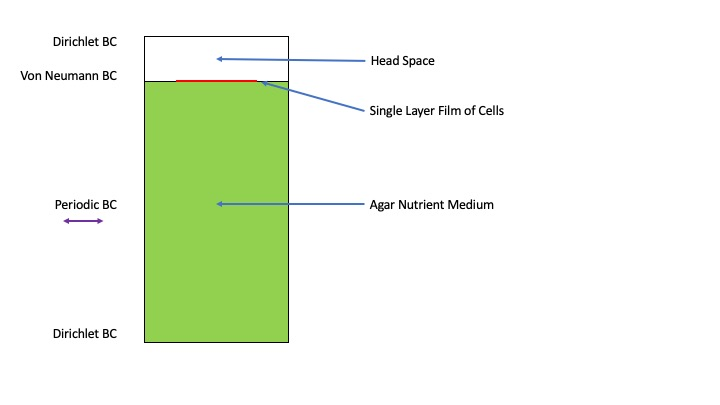
\includegraphics[width=4.0in,keepaspectratio=true]{FullSys}
\caption{\label{fullsys} Schematic diagram of the model growth region.}
\end{figure}
The geometry of the system is illustrated in figure (\ref{fullsys}) and shows a
rectangular volume that is square in cross section and elongated along one axis.
the system is periodic along the short axes. The long axis is divided into two
regions, one consisting of the stationary growth region and the other consisting
of a non-participating ``head-space''. The nutrient concentration is maintained
at a fixed value at the bottom of the system, corresponding to a Dirichlet
boundary condition. The top of the growth medium is impermeable to the nutrient,
so it should be characterized by a Von Neumann boundary condition representing
a zero normal gradient for the nutrient concentration. The head space does not
contain any chemical species and for this problem does not participate in any
significant way. The cells grow on top of the nutrient support layer in a
two-dimensional pattern.

\begin{figure}
\centering
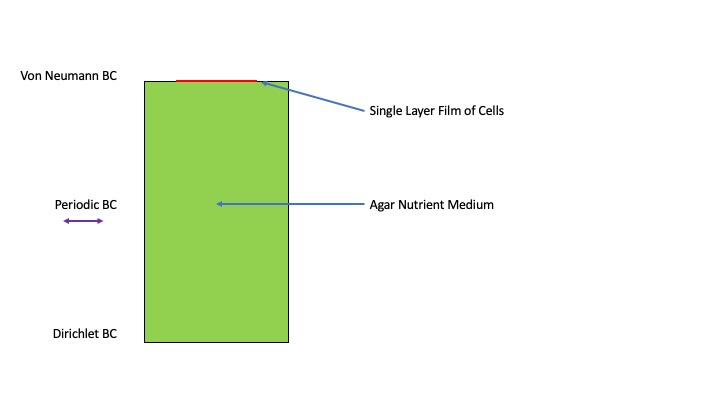
\includegraphics[width=4.0in,keepaspectratio=true]{ReducedSys}
\caption{\label{reducedsys} Schematic diagram of the model growth region with
head space removed.}
\end{figure}
Because the head space does not participate in any substantial way in this
model, it is possible to eliminate it entirely and use the geometry shown in
figure (\ref{reducedsys}). This eliminates an internal boundary and should make
development easier, but may gloss over an issue that will need to be dealt with
later as the model becomes more realistic.

\begin{figure}
\centering
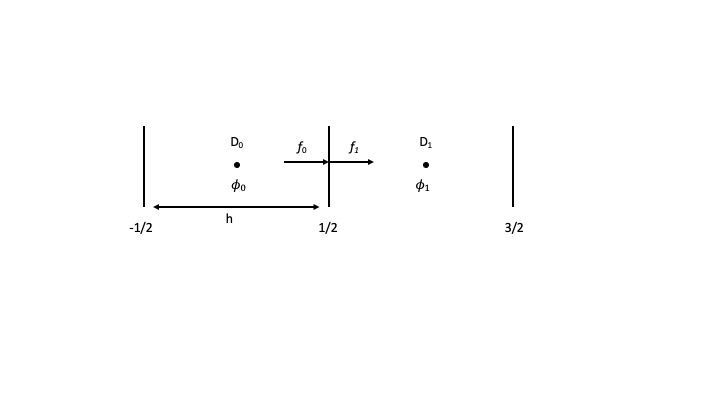
\includegraphics[width=4.0in,keepaspectratio=true]{DiffBC}
\caption{\label{diffbc} Illustration of the geometry for solving the boundary
conditions between two media with different diffusion coefficients.}
\end{figure}
In the case that there is an internal boundary, the finite volume approach can
be used incorporate the effects of the jump in diffusion coefficient. For
simplicity, consider a 1-dimensional system with evenly spaced grid cells of
size $h$. The centers of the grid cells are indexed by the integers $i$ and the
faces between the cells are indexed by $i+1/2$. Consider two grid cells at $i=0$
and $i=1$ and assume that the boundary between them at $i=1/2$ is where the
diffusion coefficient changes abruptly from the value $D_0$ to $D_1$. The
cell-centered concentration values are $\phi_0$ and $\phi_1$. The system is
illustrated schematically in figure (\ref{diffbc})

To derive the boundary condition, assume that the concentration field $\phi$ is
continuous at the boundary and has the unknown value $\phi_{1/2}$. This value
can be determined by the requirement that the fluxes calculated on both sides of
the boundary must be equal. The diffusive flux $f$ has the form
\[
f =-D\hat{n}\cdot\nabla\phi
\]
where $\hat{n}$ is a unit normal to the surface.

Using a standard finite difference calculation for the discrete form for the
gradient, the equality of the fluxes $f_0=f_1$ on both sides of the boundary at $i=1/2$
becomes
\[
-\frac{\phi_{1/2}-\phi_0}{h/2}D_0 = -\frac{\phi_{1}-\phi_{1/2}}{h/2}D_1
\]
This equation is readily solved for $\phi_{1/2}$ in terms of $\phi_0$ and
$\phi_1$ to get the weighted average
\[
\phi_{1/2} = \frac{D_0\phi_0+D_1\phi_1}{D_0+D_1}
\]
Substituting this result back into formulas for the fluxes gives
\[
f_0=f_1=-2\frac{D_0 D_1}{D_0+D_1}\frac{\phi_1-\phi_0}{h}
\]
This formula is very interesting and suggest that if diffusion coefficients are
defined on the faces of grid cells, then a step discontinuity in the value of
the diffusion coefficient in two cells can be handle by using the value
\[
2\frac{D_0 D_1}{D_0+D_1}
\]
on the face seperating the two cells.

\section{Biological Cell Dynamics}
This model will employ a very simple set of equations to describe dynamics within the
cell. Three chemical constituents are considered, $A$, $B$ and $C$. $A$ and $C$ exist
both inside and outside the cell (in the agar medium) and the concentrations outside
the cell are denoted with the subscript $out$ and those inside the cell are labeled
with the subscript $in$. The compound $B$ is only located inside the cell. These species
are related to each other as follows:
\begin{eqnarray*}
A_{out} &\stackrel{k_{1},k_{-1}}{\longleftrightarrow}& A_{in} \\
A_{in} &\stackrel{k_2,k_{-2}}{\longleftrightarrow}& B_{in} + C_{in} \\
C_{in} &\stackrel{k_3,k_{-3}}{\longleftrightarrow}& C_{out}
\end{eqnarray*}
The intracellular concentration of these species is governed by the set of equations
\begin{eqnarray*}
\frac{\partial A_{out}}{\partial t} &=&-k_1 A_{out}+k_{-1} A_{in} \\
\frac{\partial A_{in}}{\partial t} &=&k_1 A_{out}-k_{-1} A_{in} - k_2 A_{in}
 - k_{-2}B_{in}C_{in}\\
\frac{\partial B_{in}}{\partial t} &=&k_2 A_{in} - k_{-2}B_{in}C_{in}\\
\frac{\partial C_{in}}{\partial t} &=&k_2 A_{in} - k_{-2}B_{in}C_{in}-k_3 C_{in}
+ k_{-3} C_{out} \\
\frac{\partial C_{out}}{\partial t} &=&k_3 C_{in}-k_{-3} C_{out}
\end{eqnarray*}
The cells are subject to two additional rules:
\begin{list}{$\bullet$}{}
\item If $\partial B_{in}/\partial t$ falls to zero, the cell dies.
\item If $\partial B_{in}/\partial t$ and the amount of $B_{in}$ increases to 10, the
cell splits into two new cells.
\end{list}
These reactions also act as sources and sinks for $A_{in}$ and $C_{in}$, which are governed
by diffusion in the agar growth medium.

Some additional questions:
\begin{list}{$\bullet$}{}
\item What are the rules governing mechanical interactions between the cells?
\item Is their a growth rule for the cells e.g. $\partial V/\partial t = f(A_{in},
B_{in},C_{in})$ or possibly $\partial V/\partial t = f(\partial A_{in}/\partial t,
\partial B_{in}/\partial t, \partial C_{in}/\partial t)$?
\item What are initial conditions, both inside and outside the cell?
\end{list}
\end{document}
